\section{Explanation methods}
\label{appendix: Explanation methods}

\textbf{Gradient} is a common back-propagation based method which directly uses the gradients of the output logit as explanation, defined as $\phi^t(\mathbf{x})_y = \nabla_\textbf{x}y^t$.

\textbf{GradCam} is a class-discriminative localization technique that can be used for any CNN model \citep{gradcam}. GradCAM uses the gradients of the class score, before the softmax, with respect to the feature map activation of the final convolutional layer. Next, the gradients obtained are globally average-pooled across each feature map. This effectively summarizes the importance of each feature map, determining the importance of each feature map in the final classification decision. These weights are then linearly combined with the corresponding feature maps. Finaly, the ReLU activation function is applied to remove all negative pixels, which are likely to be important to other categories of the image. GradCAM are defined as

\begin{equation}
\phi^t(\mathbf{x})_y = ReLU(\sum_k( \frac{1}{z} \sum_{i,j} \frac{\partial y^t}{\partial A^k_{ij}} ) A^k )
\end{equation}

where $i,j$ are the spatial coordinates and $z$ are the total number of coordinates. $y^t$ is the logit score with respect to class t, and $A^k$ is the feature map activation of channel $k$. $\frac{\partial y^c}{\partial A^k_{ij}}$ are the gradients, $\frac{1}{z} \sum_{i,j}$ the global average-pooling and $\sum_k(\alpha A^k)$ the weighted linear combination of the feature maps and weights.

\textbf{Linear Approximation} is a method implemented by \texttt{TorchRay}\footnote{See, \href{https://facebookresearch.github.io/TorchRay/attribution.html\#module-torchray.attribution.linear\_approx}{https://facebookresearch.github.io/TorchRay/attribution.html\#module-torchray.attribution.linear\_approx}.}. It creates the explanation map by calculateing the element-wise product of feature and gradients. This gives the explanation

\begin{equation}
    \phi^t(\mathbf{x})_y = A^k \odot \nabla_{A^k}y^t
\end{equation}

where $y^t$ is the logit score with respect to class t, and $A^k$ the feature map activation of channel $k$.

\clearpage
\section{Additional results}
\label{app:add_res}

\begin{figure}[h]
\begin{tabular}{c c c}
    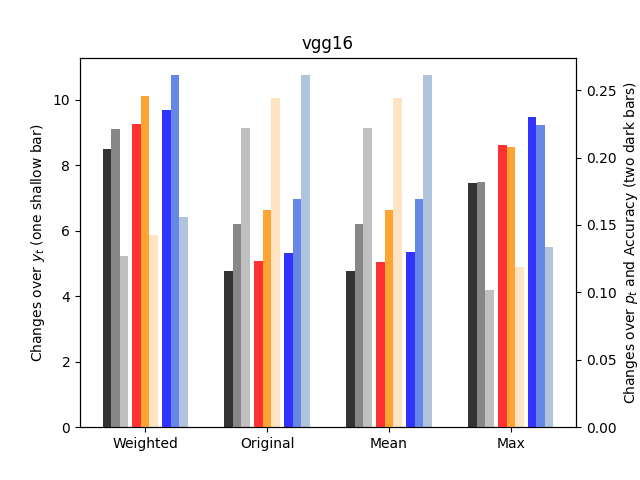
\includegraphics[width = 0.3\textwidth]{figures/grad_sign_perturbation/vgg16_eps001.png} &
    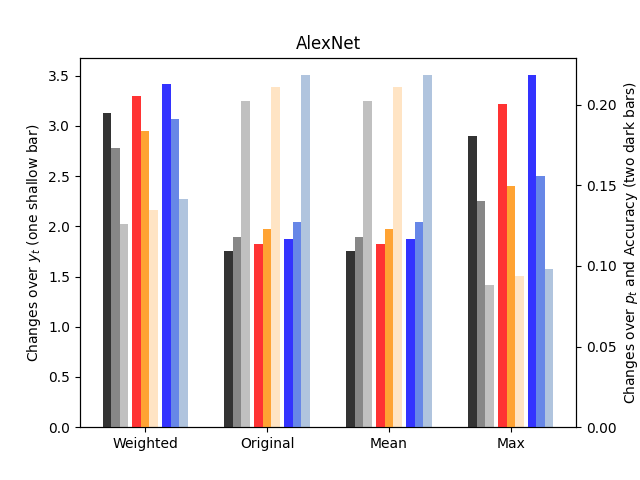
\includegraphics[width = 0.3\textwidth]{figures/grad_sign_perturbation/alexnet_eps001.png} &
    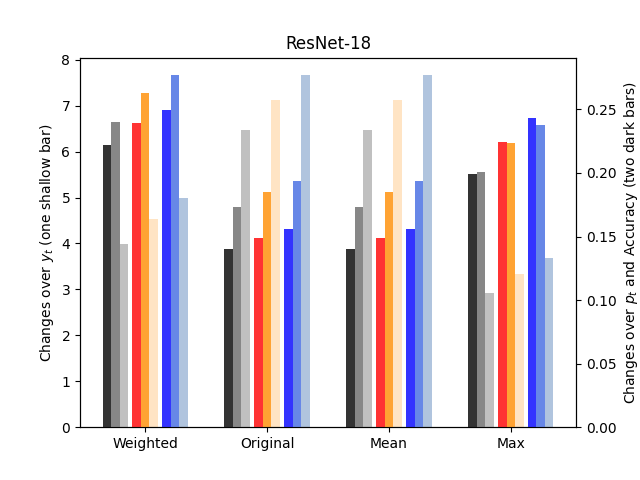
\includegraphics[width = 0.3\textwidth]{figures/grad_sign_perturbation/resnet18_eps001.png} \\

    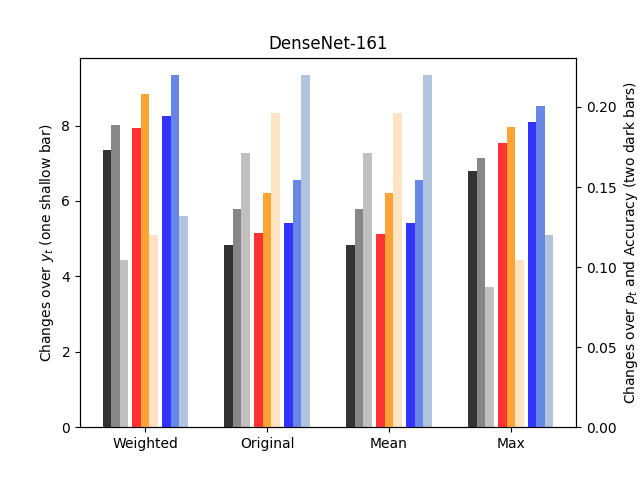
\includegraphics[width = 0.3\textwidth]{figures/grad_sign_perturbation/densenet161_eps001.png} &
    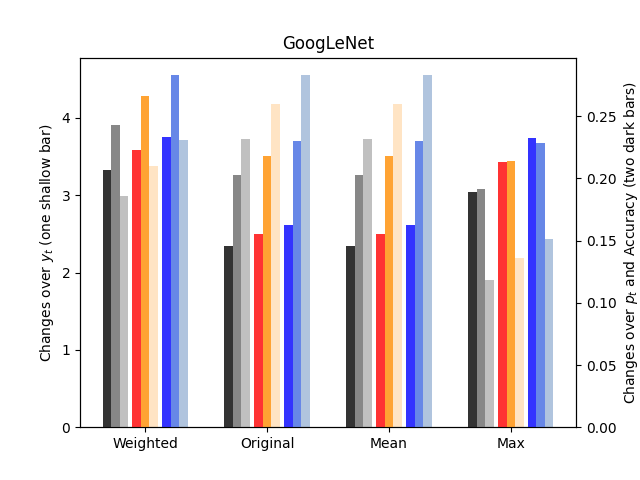
\includegraphics[width = 0.3\textwidth]{figures/grad_sign_perturbation/googlenet_eps001.png} &
    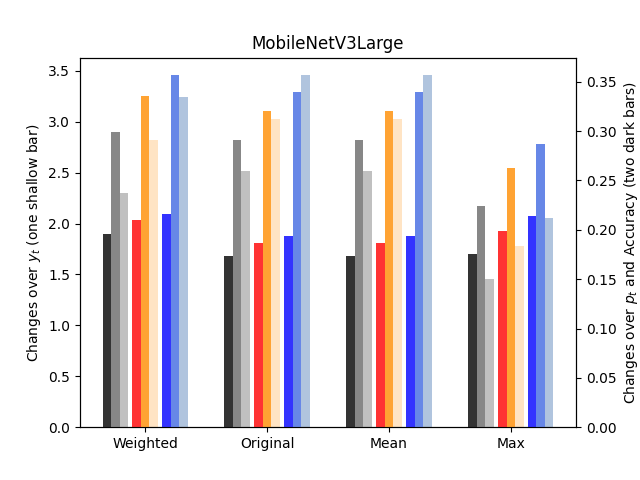
\includegraphics[width = 0.3\textwidth]{figures/grad_sign_perturbation/mobilenetv3large_eps001.png} \\

    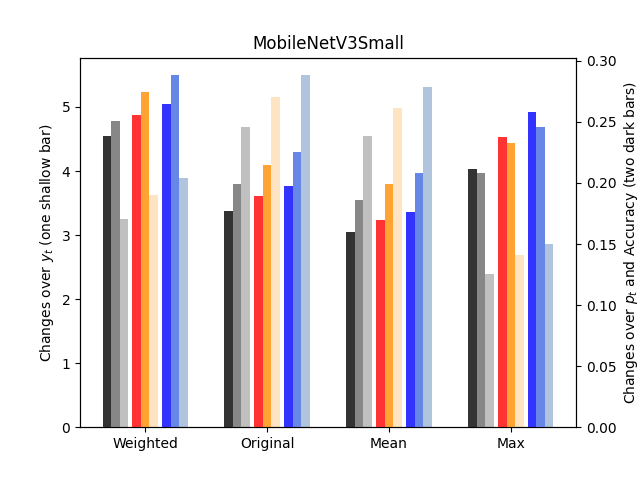
\includegraphics[width = 0.3\textwidth]{figures/grad_sign_perturbation/mobilenetv3small_eps001.png} &
    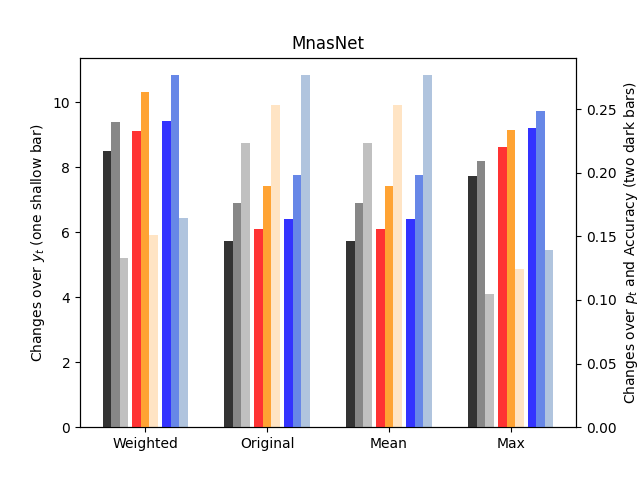
\includegraphics[width = 0.3\textwidth]{figures/grad_sign_perturbation/mnasnet_eps001.png} &
    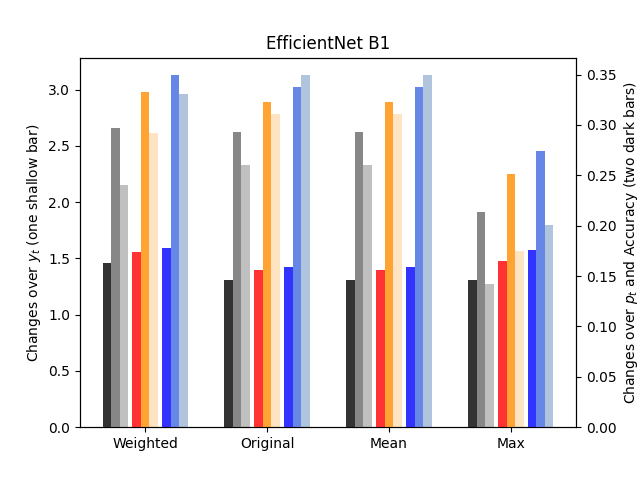
\includegraphics[width = 0.3\textwidth]{figures/grad_sign_perturbation/efficientnetB1_eps001.png} \\

\multicolumn{3}{c}{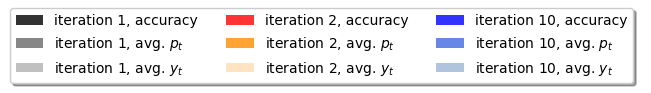
\includegraphics[width = 0.7\textwidth]{figures/grad_sign_perturbation/legend.png} }\\
\end{tabular}
\caption{Reproducing of Figure 3 in the original paper with $\epsilon=10^{-3}$. Changes in accuracy, $y_t$ and $p_t$ (t is the target classification class) when certain input features are perturbed. Perturbed features are selected based on four gradient explanations (original, mean, max and weighted), where original is directly with respect to the gradients of the logits.}
\label{f:grad_sign_perturbation_eps_001}
\end{figure}
\clearpage
\begin{figure}[t!]
\tiny
\centering

%\begin{minipage}[b]{0.48\textwidth}
\resizebox{\textwidth}{!}{\
\begin{subfigure}{.5\textwidth}
\begin{tabular}
{ 
c@{\hspace{0.09cm}} c@{\hspace{0.09cm}} c@{\hspace{0.09cm}} c@{\hspace{0.09cm}} c@{\hspace{0.09cm}}}

    % & \textbf{Original} & \text{\textbf{Standard} \\ \textbf{GradCAM}} & \textbf{GradCAM}  \textbf{wo/ ReLU} & \textbf{Contrastive} \textbf{GradCAM} \\
    & \thead{Original} & \thead{Standard \\ GradCAM} & \thead{GradCAM \\ w/o ReLU} & \thead{Contrastive \\ GradCAM} \\
    
    \vspace{0.09cm}
    % $\vcenter{\hbox{Ice Cream}}$ &
    % \thead{Ice-\\cream \\ \texttt{p=0.30}} &
    $\vcenter{\hbox{\shortstack{\textbf{Ice} \textbf{cream} \\ p=0.30}}}$ &
    $\vcenter{\hbox{\includegraphics[width = \myfigurewidth\textwidth]{figures/vit-figures/icecream_l10_gradcam/original.jpg}}}$ &
    $\vcenter{\hbox{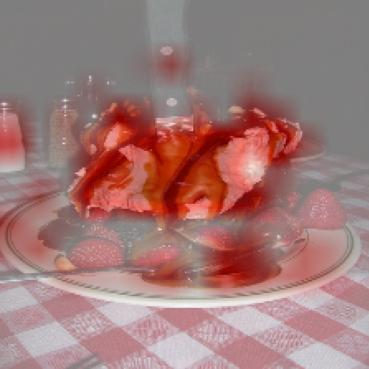
\includegraphics[width = \myfigurewidth\textwidth]{figures/vit-figures/icecream_l10_gradcam/standard_cam_w_relu.jpg}}}$ &
    $\vcenter{\hbox{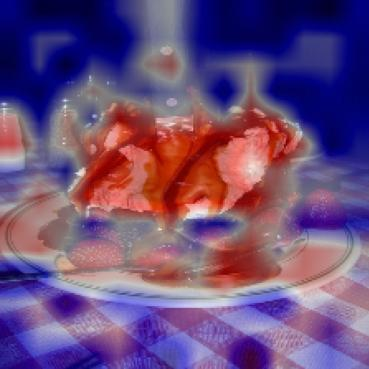
\includegraphics[width = \myfigurewidth\textwidth]{figures/vit-figures/icecream_l10_gradcam/standard_cam.jpg}}}$ &
    $\vcenter{\hbox{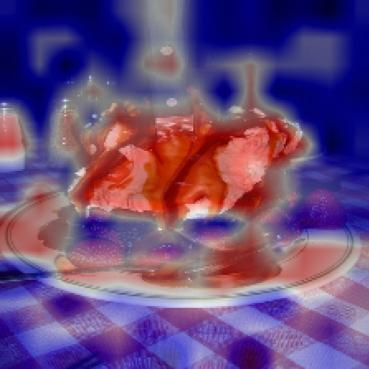
\includegraphics[width = \myfigurewidth\textwidth]{figures/vit-figures/icecream_l10_gradcam/contrastive_cam.jpg}}}$ \\

    \vspace{0.09cm}
    % \thead{Chocolate \\ Sauce} &
    $\vcenter{\hbox{\shortstack{\textbf{Chocolate} \\ \textbf{sauce} \\ p=0.30}}}$ &
    $\vcenter{\hbox{\includegraphics[width = \myfigurewidth\textwidth]{figures/vit-figures/chocolate_sauce_l10_gradcam/original.jpg}}}$ &
    $\vcenter{\hbox{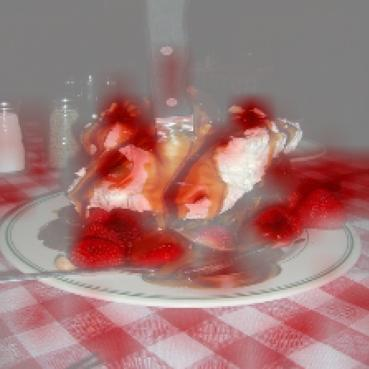
\includegraphics[width = \myfigurewidth\textwidth]{figures/vit-figures/chocolate_sauce_l10_gradcam/standard_cam_w_relu.jpg}}}$ &
    $\vcenter{\hbox{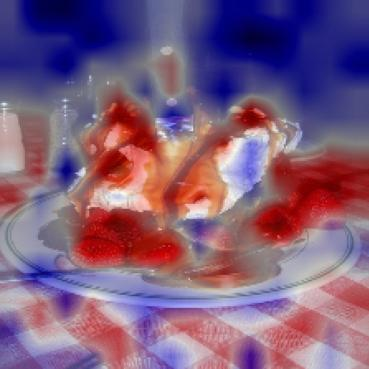
\includegraphics[width = \myfigurewidth\textwidth]{figures/vit-figures/chocolate_sauce_l10_gradcam/standard_cam.jpg}}}$ &
    $\vcenter{\hbox{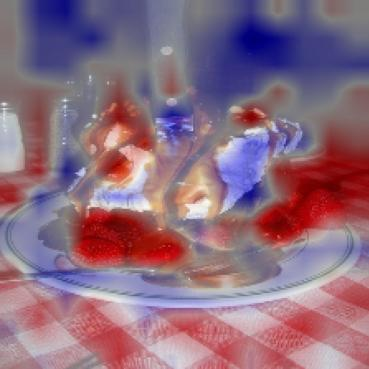
\includegraphics[width = \myfigurewidth\textwidth]{figures/vit-figures/chocolate_sauce_l10_gradcam/contrastive_cam.jpg}}}$ \\

    \vspace{0.09cm}
    % $\vcenter{\hbox{Digital Watch}}$ &
    % \thead{Digital \\ Watch} &
    $\vcenter{\hbox{\shortstack{\textbf{Digital} \\ \textbf{watch} \\ p=0.32}}}$ &
    $\vcenter{\hbox{\includegraphics[width = \myfigurewidth\textwidth]{figures/vit-figures/digital_watch_l10_gradcam/original.jpg}}}$ &
    $\vcenter{\hbox{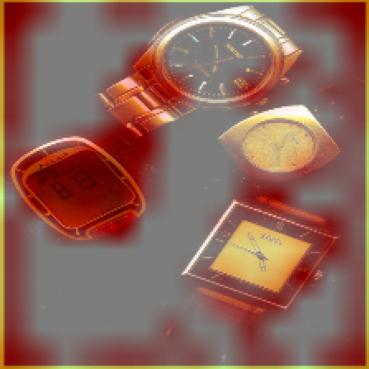
\includegraphics[width = \myfigurewidth\textwidth]{figures/vit-figures/digital_watch_l10_gradcam/standard_cam_w_relu.jpg}}}$ &
    $\vcenter{\hbox{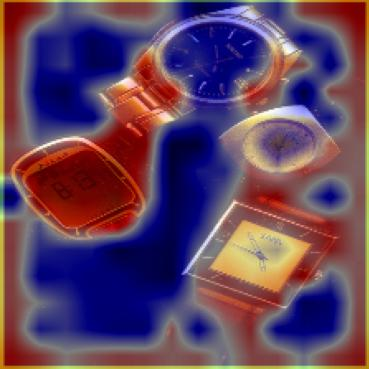
\includegraphics[width = \myfigurewidth\textwidth]{figures/vit-figures/digital_watch_l10_gradcam/standard_cam.jpg}}}$ &
    $\vcenter{\hbox{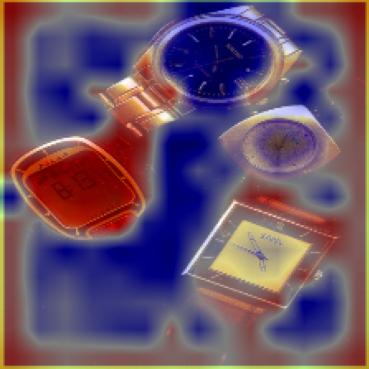
\includegraphics[width = \myfigurewidth\textwidth]{figures/vit-figures/digital_watch_l10_gradcam/contrastive_cam.jpg}}}$ \\

    \vspace{0.09cm}
    % $\vcenter{\hbox{Stopwatch}}$ &
    % \thead{Stop-\\watch} &
    $\vcenter{\hbox{\shortstack{\textbf{Stopwatch} \\ p=0.32}}}$ &
    $\vcenter{\hbox{\includegraphics[width = \myfigurewidth\textwidth]{figures/vit-figures/stopwatch_l10_gradcam/original.jpg}}}$ &
    $\vcenter{\hbox{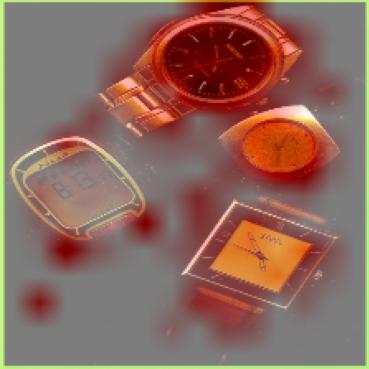
\includegraphics[width = \myfigurewidth\textwidth]{figures/vit-figures/stopwatch_l10_gradcam/standard_cam_w_relu.jpg}}}$ &
    $\vcenter{\hbox{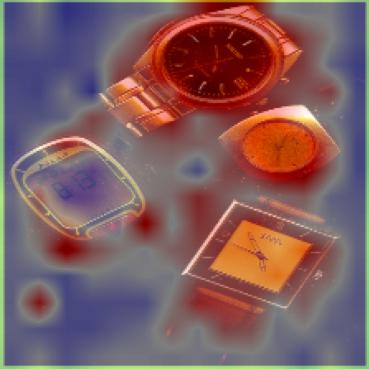
\includegraphics[width = \myfigurewidth\textwidth]{figures/vit-figures/stopwatch_l10_gradcam/standard_cam.jpg}}}$ &
    $\vcenter{\hbox{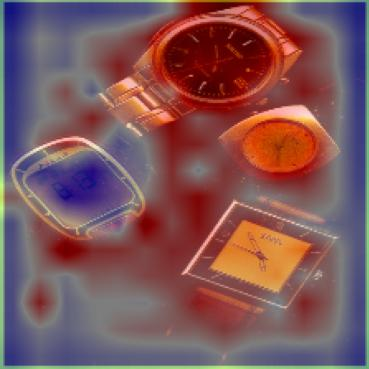
\includegraphics[width = \myfigurewidth\textwidth]{figures/vit-figures/stopwatch_l10_gradcam/contrastive_cam.jpg}}}$ \\  

\end{tabular}
\caption{} \label{t:}
\label{fig:vit-gradcam}
\end{subfigure}

\begin{subfigure}{.5\textwidth}
\begin{tabular}
{ 
c@{\hspace{0.09cm}} c@{\hspace{0.09cm}} c@{\hspace{0.09cm}} c@{\hspace{0.09cm}} c@{\hspace{0.09cm}}}
    & \thead{Original} & \thead{Gradient-\\weighted \\ Attention \\ Rollout} & \thead{Gradient-\\ weighted \\ Attention \\ Rollout \\ w/o ReLU} & \thead{Contrastive \\ Gradient-\\weighted \\ Attention \\ Rollout} \\
    
    \vspace{0.09cm}
    $\vcenter{\hbox{\shortstack{\textbf{Ice} \textbf{cream} \\ p=0.30}}}$ &
    $\vcenter{\hbox{\includegraphics[width = \myfigurewidth\textwidth]{figures/vit-figures/attention_rollout/icecream/original.png}}}$ &
    $\vcenter{\hbox{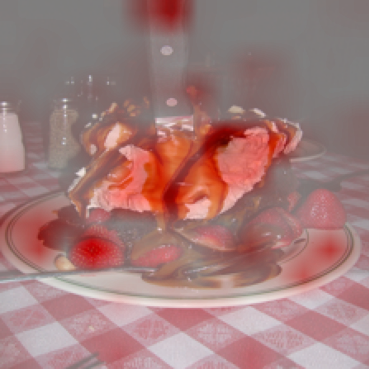
\includegraphics[width = \myfigurewidth\textwidth]{figures/vit-figures/attention_rollout/icecream/standard.png}}}$ &
    $\vcenter{\hbox{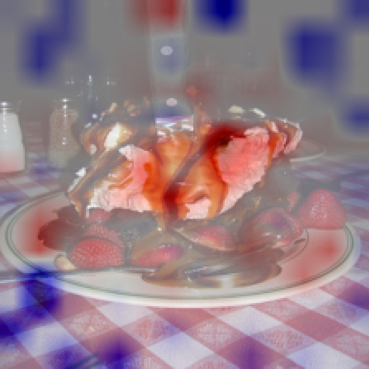
\includegraphics[width = \myfigurewidth\textwidth]{figures/vit-figures/attention_rollout/icecream/standard_contrastive.png}}}$ &
    $\vcenter{\hbox{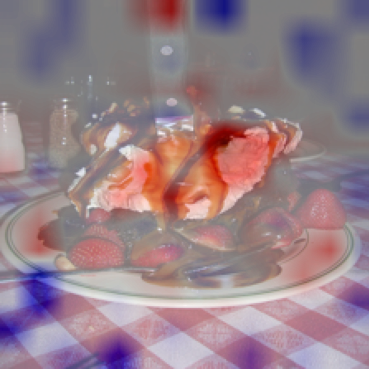
\includegraphics[width = \myfigurewidth\textwidth]{figures/vit-figures/attention_rollout/icecream/contrastive.png}}}$ \\

    \vspace{0.09cm}
    $\vcenter{\hbox{\shortstack{\textbf{Chocolate} \\ \textbf{sauce} \\ p=0.30}}}$ &
    $\vcenter{\hbox{\includegraphics[width = \myfigurewidth\textwidth]{figures/vit-figures/attention_rollout/chocolate/original.png}}}$ &
    $\vcenter{\hbox{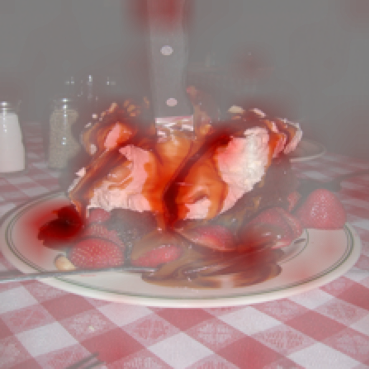
\includegraphics[width = \myfigurewidth\textwidth]{figures/vit-figures/attention_rollout/chocolate/standard.png}}}$ &
    $\vcenter{\hbox{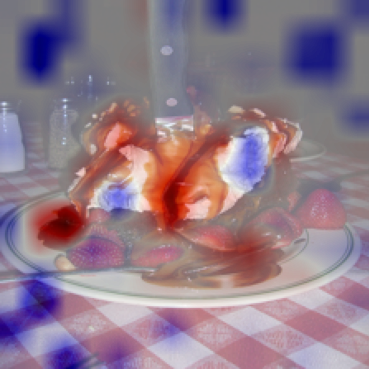
\includegraphics[width = \myfigurewidth\textwidth]{figures/vit-figures/attention_rollout/chocolate/standard_contrastive.png}}}$ &
    $\vcenter{\hbox{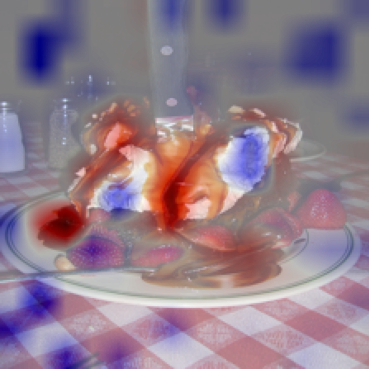
\includegraphics[width = \myfigurewidth\textwidth]{figures/vit-figures/attention_rollout/chocolate/contrastive.png}}}$ \\

    \vspace{0.09cm}
    $\vcenter{\hbox{\shortstack{\textbf{Digital} \\ \textbf{watch} \\ p=0.32}}}$ &
    $\vcenter{\hbox{\includegraphics[width = \myfigurewidth\textwidth]{figures/vit-figures/attention_rollout/digital/original.png}}}$ &
    $\vcenter{\hbox{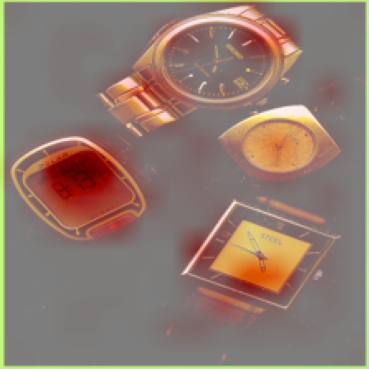
\includegraphics[width = \myfigurewidth\textwidth]{figures/vit-figures/attention_rollout/digital/standard.png}}}$ &
    $\vcenter{\hbox{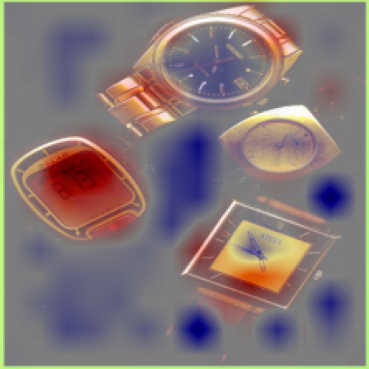
\includegraphics[width = \myfigurewidth\textwidth]{figures/vit-figures/attention_rollout/digital/standard_contrastive.png}}}$ &
    $\vcenter{\hbox{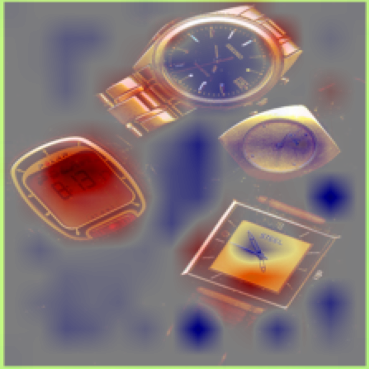
\includegraphics[width = \myfigurewidth\textwidth]{figures/vit-figures/attention_rollout/digital/contrastive.png}}}$ \\

    \vspace{0.09cm}
    $\vcenter{\hbox{\shortstack{\textbf{Stopwatch} \\ p=0.32}}}$ &
    $\vcenter{\hbox{\includegraphics[width = \myfigurewidth\textwidth]{figures/vit-figures/attention_rollout/stopwatch/original.png}}}$ &
    $\vcenter{\hbox{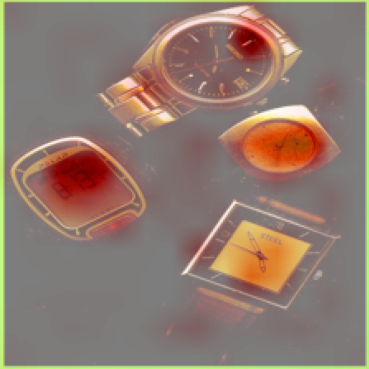
\includegraphics[width = \myfigurewidth\textwidth]{figures/vit-figures/attention_rollout/stopwatch/standard.png}}}$ &
    $\vcenter{\hbox{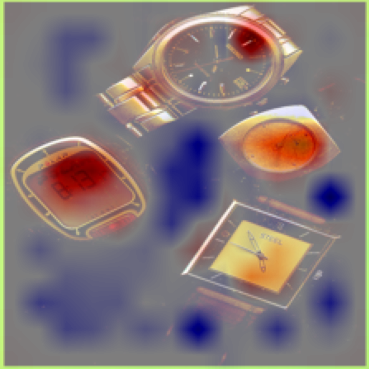
\includegraphics[width = \myfigurewidth\textwidth]{figures/vit-figures/attention_rollout/stopwatch/standard_contrastive.png}}}$ &
    $\vcenter{\hbox{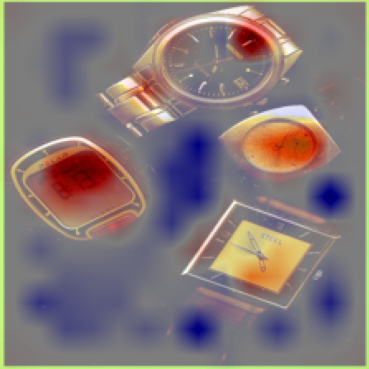
\includegraphics[width = \myfigurewidth\textwidth]{figures/vit-figures/attention_rollout/stopwatch/contrastive.png}}}$ \\

\end{tabular}
\caption{} \label{t:}
\end{subfigure}
}

\caption{Comparison between proposed ViT explanations for a pre-trained ImageNet model. In (a) a comparison between GradCAM, GradCAM without ReLU, and Contrastive GradCAM is considered. In (b) a comparison between Gradient-weighted Attention rollout (GWAR) of the standard, without ReLU, and contrastive variant is considered. Red sections are considered areas with high explainability. To adapt the method to the contrastive version all ReLU operations were removed and the gradients were calculated from the softmax output instead of the logits.} \label{t:}
\end{figure}
\null

